%%%%%%%%%%%%%%%%%%%%%%%%%%%%%%%%%%%%%%%%%%%
%
% From a template maintained at https://github.com/jamesrobertlloyd/cbl-tikz-poster
%
% Code near the top should be fairly standard and not need to be changed
%  - except for the document class
% Code lower down is more likely to be customised
%
%%%%%%%%%%%%%%%%%%%%%%%%%%%%%%%%%%%%%%%%%%%

%%%%%%%%%%%%%%%%%%%%%%%%%%%%%%%%%%%%%%%%%%%
%
% Document class
%
% Change this if you want a different size / orientation poster etc
%
%%%%%%%%%%%%%%%%%%%%%%%%%%%%%%%%%%%%%%%%%%%

%\documentclass[portrait,a0,final]{a0poster}
\documentclass[portrait,a0b,final]{a0poster}

%%%%%%%%%%%%%%%%%%%%%%%%%%%%%%%%%%%%%%%%%%%
%
% 'Basic' packages
%
% TODO - Almost certainly some are unnecessary - feel free to remove nonstandard
% packages if you think it is a good idea not to always have them
%
%%%%%%%%%%%%%%%%%%%%%%%%%%%%%%%%%%%%%%%%%%%

\usepackage{multicol}
\usepackage{color}
\usepackage{shadow}
\usepackage{morefloats}
\usepackage{cite}
\usepackage[pdftex]{graphicx}
\usepackage{rotating}
\usepackage{amsmath, amsthm, amssymb, bm}
\usepackage{array}
\usepackage{nth}
\usepackage[square,numbers]{natbib}
\usepackage{booktabs}
\usepackage[table,xcdraw]{xcolor}
%\usepackage{float}
%\usepackage{subfig}
%\usepackage{svg}
%\usepackage{wrapfig}
%\usepackage[a0paper,pass]{geometry}

%%%%%%%%%%%%%%%%%%%%%%%%%%%%%%%%%%%%%%%%%%%
%
% TIKZ packages and common definitions
%
% Add extra things as per your tikz needs
%
%%%%%%%%%%%%%%%%%%%%%%%%%%%%%%%%%%%%%%%%%%%

\usepackage{picins}
\usepackage{tikz}
\usetikzlibrary{shapes.geometric,arrows,chains,matrix,positioning,scopes,calc}
\tikzstyle{mybox} = [draw=white, rectangle]

%%%%%%%%%%%%%%%%%%%%%%%%%%%%%%%%%%%%%%%%%%%
%
% myfig
%
% \myfig - replacement for \figure
% necessary, since in multicol-environment 
% \figure won't work        
%                 
%%%%%%%%%%%%%%%%%%%%%%%%%%%%%%%%%%%%%%%%%%%

\newcommand{\myfig}[3][0]{
\begin{center}
  \vspace{1.5cm}
  \includegraphics[width=#3\hsize,angle=#1]{#2}
  \nobreak\medskip
\end{center}}

%%%%%%%%%%%%%%%%%%%%%%%%%%%%%%%%%%%%%%%%%%%
%
% mycaption                
%
% \mycaption - replacement for \caption
% necessary, since in multicol-environment \figure and
% therefore \caption won't work
%
%%%%%%%%%%%%%%%%%%%%%%%%%%%%%%%%%%%%%%%%%%%

%\newcounter{figure}
\setcounter{figure}{1}
\newcommand{\mycaption}[1]{
  \vspace{0.5cm}
  \begin{quote}
    {{\sc Figure} \arabic{figure}: #1}
  \end{quote}
  \vspace{1cm}
  \stepcounter{figure}
}

\newcommand{\cwicaption}[1]{
  %\vspace{0.5cm}
  \begin{quote}
    {{\sc Figure} \arabic{figure}: #1}
  \end{quote}
  %\vspace{1cm}
  \stepcounter{figure}
}

%%%%%%%%%%%%%%%%%%%%%%%%%%%%%%%%%%%%%%%%%%%
%
% Some standard colours
%
%%%%%%%%%%%%%%%%%%%%%%%%%%%%%%%%%%%%%%%%%%%

\definecolor{camlightblue}{rgb}{0.601 , 0.8, 1}
\definecolor{camdarkblue}{rgb}{0, 0.203, 0.402}
\definecolor{camred}{rgb}{1, 0.203, 0}
\definecolor{camyellow}{rgb}{1, 0.8, 0}
\definecolor{lightblue}{rgb}{0, 0, 0.80}
\definecolor{white}{rgb}{1, 1, 1}
\definecolor{whiteblue}{rgb}{0.80, 0.80, 1}
\definecolor{cwired}{rgb}{0.803,0.0,0.227}

%%%%%%%%%%%%%%%%%%%%%%%%%%%%%%%%%%%%%%%%%%%
%
% Some look and feel definitions
%
%%%%%%%%%%%%%%%%%%%%%%%%%%%%%%%%%%%%%%%%%%%

\setlength{\columnsep}{0.03\textwidth}
\setlength{\columnseprule}{0.0018\textwidth}
\setlength{\parindent}{0.0cm}

%%%%%%%%%%%%%%%%%%%%%%%%%%%%%%%%%%%%%%%%%%%
%
% \mysection - replacement for \section*
% 
% Puts a pretty box around some text
% TODO - any other thoughts for what this box should look like
%
%%%%%%%%%%%%%%%%%%%%%%%%%%%%%%%%%%%%%%%%%%%

\tikzstyle{mysection} = [rectangle, 
						draw=none, 
						shade, 
						outer color=cwired,
						inner color=cwired,
						text width=0.9\columnwidth,
						text centered,
						rounded corners=20pt,
						minimum height=0.11\columnwidth]

\newcommand{\mysection}[1]
{
\begin{center}
  \begin{tikzpicture}
    \node[mysection,white] {\sffamily\bfseries\LARGE#1};
  \end{tikzpicture}
\end{center}
}

%%%%%%%%%%%%%%%%%%%%%%%%%%%%%%%%%%%%%%%%%%%
%
% Set the font
%
% TODO - Not sure what a canonical choice is - feel free to modify
%
%%%%%%%%%%%%%%%%%%%%%%%%%%%%%%%%%%%%%%%%%%%

\renewcommand{\familydefault}{cmss}
\sffamily

%%%%%%%%%%%%%%%%%%%%%%%%%%%%%%%%%%%%%%%%%%%
%
% Poster environment
%
% Centres everything and can be used to define the width of the content
%
%%%%%%%%%%%%%%%%%%%%%%%%%%%%%%%%%%%%%%%%%%%

\newenvironment{poster}{
  \begin{center}
  \begin{minipage}[c]{0.85\textwidth}
}{
  \end{minipage} 
  \end{center}
}

%%%%%%%%%%%%%%%%%%%%%%%%%%%%%%%%%%%%%%%%%%%
%
% This is probably a good place to put content specific packages and definitions
%
%%%%%%%%%%%%%%%%%%%%%%%%%%%%%%%%%%%%%%%%%%%

%%%%%%%%%%%%%%%%%%%%%%%%%%%%%%%%%%%%%%%%%%%
%
% The document environment starts here
%
%%%%%%%%%%%%%%%%%%%%%%%%%%%%%%%%%%%%%%%%%%%

\begin{document}

%%%%%%%%%%%%%%%%%%%%%%%%%%%%%%%%%%%%%%%%%%%
%
% Begin the poster environment - centres things and potentially changes the width
%
%%%%%%%%%%%%%%%%%%%%%%%%%%%%%%%%%%%%%%%%%%%

\begin{poster}

%%%%%%%%%%%%%%%%%%%%%%%%%%%%%%%%%%%%%%%%%%%
%
% Potentially add some space at the top of the poster
%
%%%%%%%%%%%%%%%%%%%%%%%%%%%%%%%%%%%%%%%%%%%

\vspace{0\baselineskip}

%%%%%%%%%%%%%%%%%%%%%%%%%%%%%%%%%%%%%%%%%%%
%
% Draw the header as a TIKZ picture
%
% Using TIKZ to allow for easy alignment
%
%%%%%%%%%%%%%%%%%%%%%%%%%%%%%%%%%%%%%%%%%%%

\begin{center}
\begin{tikzpicture}[x=0.5\textwidth]
    % Dummy nodes at edges for spacing
    % TODO - a better way?
    \node at (+1, 0) {};    
    \node at (-1, 0) {};
    % Set the size of the badges
    \def \badgeheight {0.08\textwidth}
    % Title text
    \node[inner sep=0,text width=0.5\textwidth,text centered,font=\Huge] (Title) at (0,0) 
    {
        {\sffamily\Huge \textbf{Geomagnetic activity, Space Weather and Machine Learning}}\\
        {\sffamily\huge Mandar Chandorkar, Enrico Camporeale}\\
        \vspace{-0.3\baselineskip}
        {\sffamily\large Multiscale Dynamics, CWI}
    };
    % Cambridge badge
    \node [mybox] (CWI Logo) at (-0.9, 0) {
        
\includegraphics[height=\badgeheight]{cwi-logo.png}
    };
    % CBL badge
    \node [mybox] (Inria logo) at (+0.7, 0) {
        
\includegraphics[height=\badgeheight]{inria-logo.jpg}
    };
\end{tikzpicture}
\end{center}

%%%%%%%%%%%%%%%%%%%%%%%%%%%%%%%%%%%%%%%%%%%
%
% Spacing between title and main body
%
%%%%%%%%%%%%%%%%%%%%%%%%%%%%%%%%%%%%%%%%%%%

\vspace{\baselineskip}

%%%%%%%%%%%%%%%%%%%%%%%%%%%%%%%%%%%%%%%%%%%
%
% Columns environment
%
%%%%%%%%%%%%%%%%%%%%%%%%%%%%%%%%%%%%%%%%%%%

\begin{multicols}{2}

%%%%%%%%%%%%%%%%%%%%%%%%%%%%%%%%%%%%%%%%%%%
%
% Start of content
%
%%%%%%%%%%%%%%%%%%%%%%%%%%%%%%%%%%%%%%%%%%%

%\large

\mysection{Space Weather}

%\myfig{nasa-space-weather}{0.5}
%\mycaption{Impacts of Space Weather phenomena}

Space weather is a branch of space physics concerned with the time varying conditions within the Solar System, including the solar wind, emphasizing the space surrounding the Earth, including conditions in the magnetosphere and ionosphere.

\myfig{magnetosphere}{1.0}
\mycaption{Space Weather Drivers and Dynamics}

\begin{itemize}
\item The sun is the main driver of space weather. Bursts of plasma from the sun's atmosphere called coronal mass ejections (CME) together with sudden bursts of radiation, all cause space weather effects here on Earth.
\item Coronal Mass Ejections (CMEs) can cause Geomagnetic Storms at Earth and induce extra currents in the ground that can affect power grid operations.
\item Geomagnetic storms can also modify the signal from radio navigation systems (GPS and GNSS) causing degraded accuracy and produce aurora. 
\end{itemize}

\vspace{\baselineskip}
\mysection{Geomagnetic Activity and Indexes}
\myfig{dst}{1.0}
\mycaption{Dst as a time series}

Due to the complex nature of the governing dynamics of geo-magnetic response to driving forces (solar wind), it is useful to use representative indexes to record and predict activity of the magnetosphere. The Dst index is an index of magnetic activity derived from a network of near-equatorial geomagnetic observatories that measures the intensity of the globally symmetrical equatorial electro-jet (the "ring current"). Dst is maintained at the National Geo-physical Data Center (NGDC) and is available via FTP from 1957 to the present.

\vspace{\baselineskip}
\mysection{Dst Models: Gaussian Process Regression}

In existing scientific literature, machine learning based predictive models for geomagnetic indexes can be classified as follows.

\begin{itemize}
    \item Non-linear auto-regressive
    \item Neural Network based
    \item Bayesian inference
\end{itemize}

In the Bayesian inference category, Gaussian Process models are quite robust and have not been utilized in space weather prediction. 

\vspace{\baselineskip}

\myfig{gp}{0.45} 
\mycaption{A function drawn from a Gaussian Process prior}

\textit{Gaussian Process} (GP) models specify statistical distributions over functions, which can be designed by choosing appropriate covariance structures to model data. Estimates produced by such models are non-parametric in nature and are akin to fitting smoothing splines to data points. In GP models, the finite dimensional distribution of the output data is a multivariate Gaussian specified by equation \ref{eq:gp}

\begin{align}
& y = f(x) + \epsilon \\
& f \sim \mathcal{GP}(m(x), C(x,x^{'})) \\
& \left(\mathbf{y} \ \ \mathbf{f_*} \right)^T \sim 
\mathcal{N}\left(\mathbf{0}, \left[ \begin{matrix} K(X, X) + \sigma^{2}_n \it{I} & K(X, X_*) \\ K(X_*, X) & K(X_*, X_*) \end{matrix} \right ] \right) 
\label{eq:gp}
\end{align}

\begin{align}
& \mathbf{f_*}|X,\mathbf{y},X_* \sim \mathcal{N}(\mathbf{\bar{f_*}}, cov(\mathbf{f_*}))  \\
& \mathbf{\bar{f_*}} \overset{\triangle}{=} \mathbb{E}[\mathbf{f_*}|X,y,X_*] = K(X_*,X)[K(X,X) + \sigma^{2}_n \it{I}]^{-1} \mathbf{y}  \\
& cov(\mathbf{f_*}) = K(X_*,X_*) - K(X_*,X)[K(X,X) + \sigma^{2}_n \it{I}]^{-1}K(X,X_*) 
\label{eq:posterior}
\end{align}

In order to make predictions using GP models, one must calculate the posterior predictive distribution $\mathbf{f_*}|X,\mathbf{y},X_*$ which is also a multi-variate Gaussian shown in equation \ref{eq:posterior}.
\vspace{\baselineskip}
\mysection{Dst Gaussian Process: FBM versus RBF kernel}

\begin{align}
    & Dst(v) \sim \mathcal{GP}(m(v), C(u,v)) \label{eq:DstGP}\\
    & C_{rbf}(u,v) = \mathbb{E}[Dst(u) \times Dst(v)] =  e^{-\frac{1}{2}|u-v|^2/\sigma^2} \label{eq:rbfcov}\\
    & C_{fbm}(u,v) = \mathbb{E}[Dst(u) \times Dst(v)] = |u|^{2H} + |v|^{2H} - |u-v|^{2H} \label{eq:fbmcov}
\end{align}

Using the solar wind speed as a predictive variable, we train a Gaussian Process model to predict the Dst index \ref{eq:DstGP}. We compare the regression performance of the \textit{Radial Basis Function} (RBF) kernel versus the \textit{Fractional Brownian Motion} (FBM) kernel (eq. \ref{eq:rbfcov},\ref{eq:fbmcov}). $H \ \in (0,1]$ and $\sigma$ are the hyper-parameters of the FBM and RBF kernels respectively.


\begin{tabular}{ll}
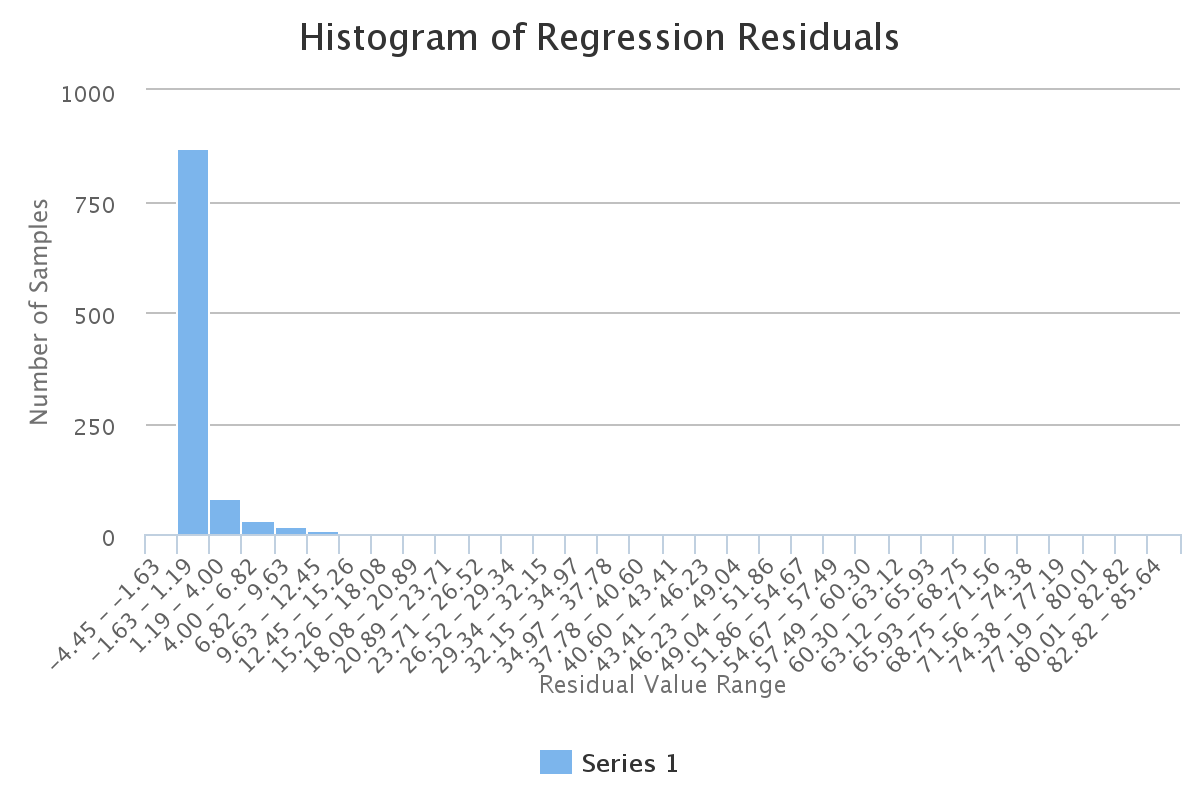
\includegraphics[width=0.45\hsize]{rbf-hist} & 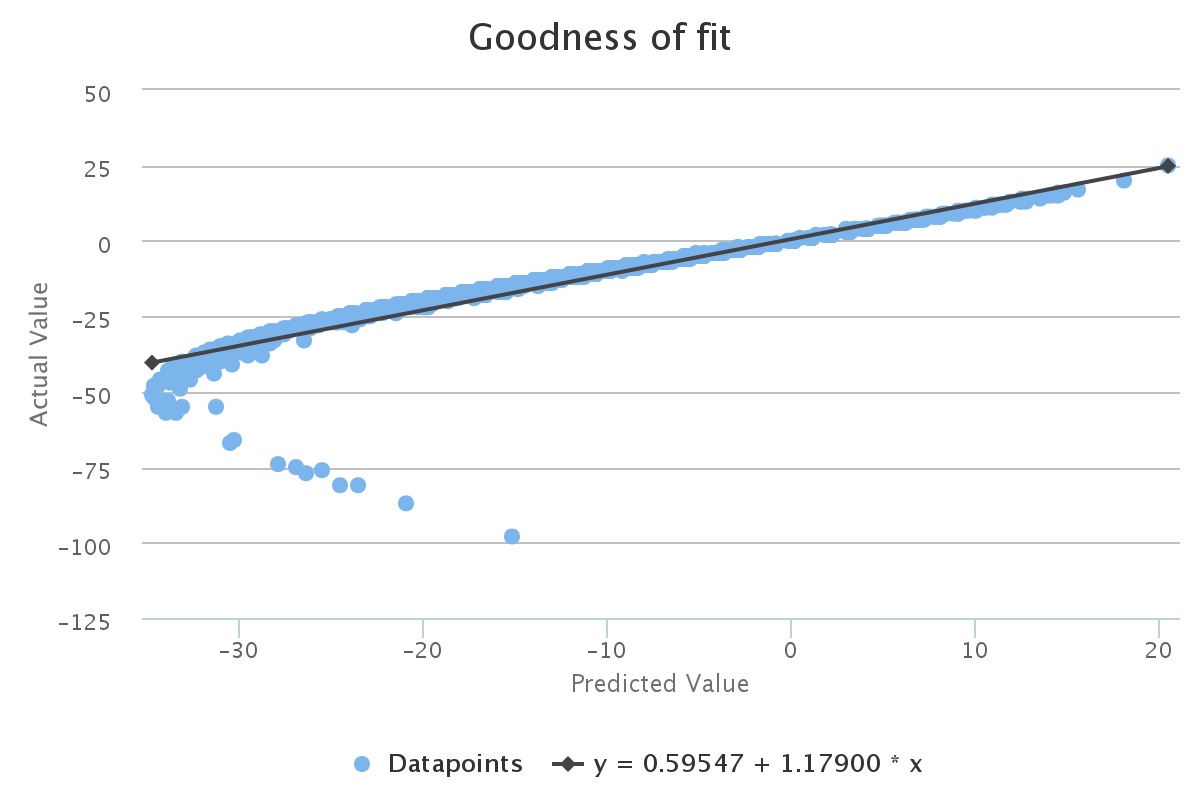
\includegraphics[width=0.45\hsize]{rbf-fit}   \\
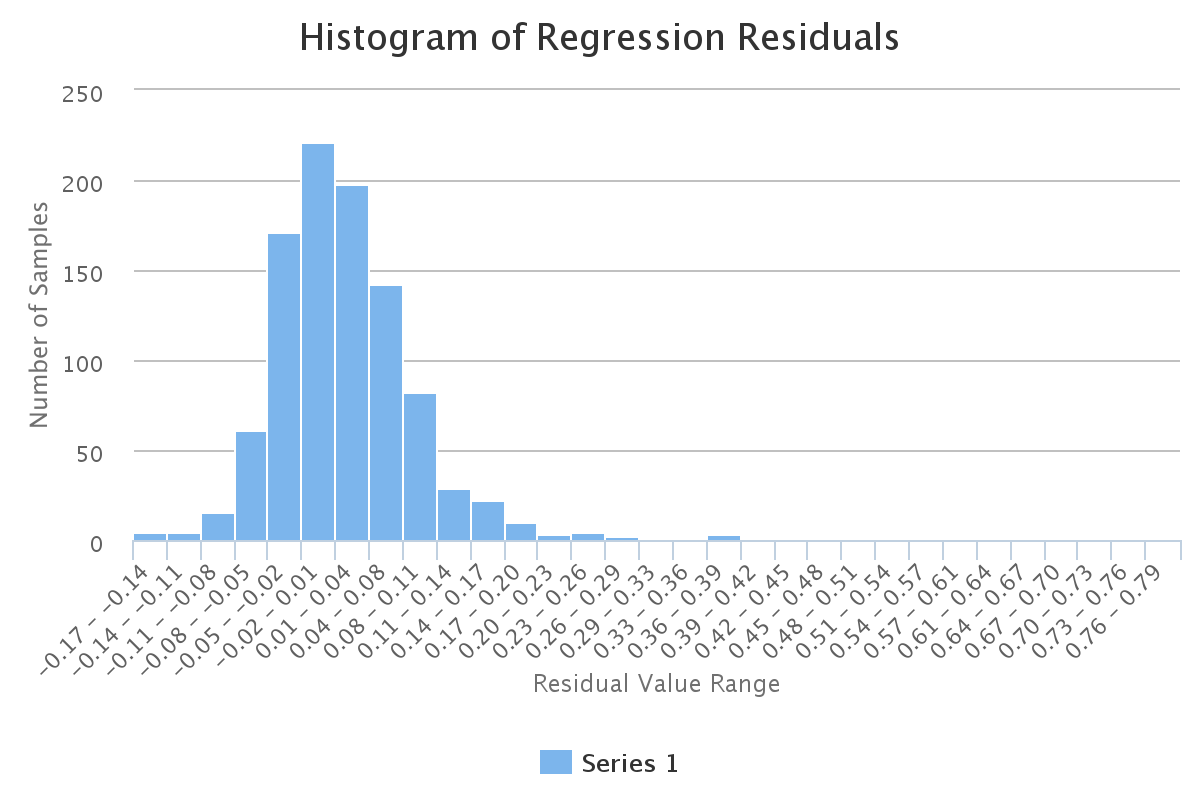
\includegraphics[width=0.45\hsize]{fbm-hist} & 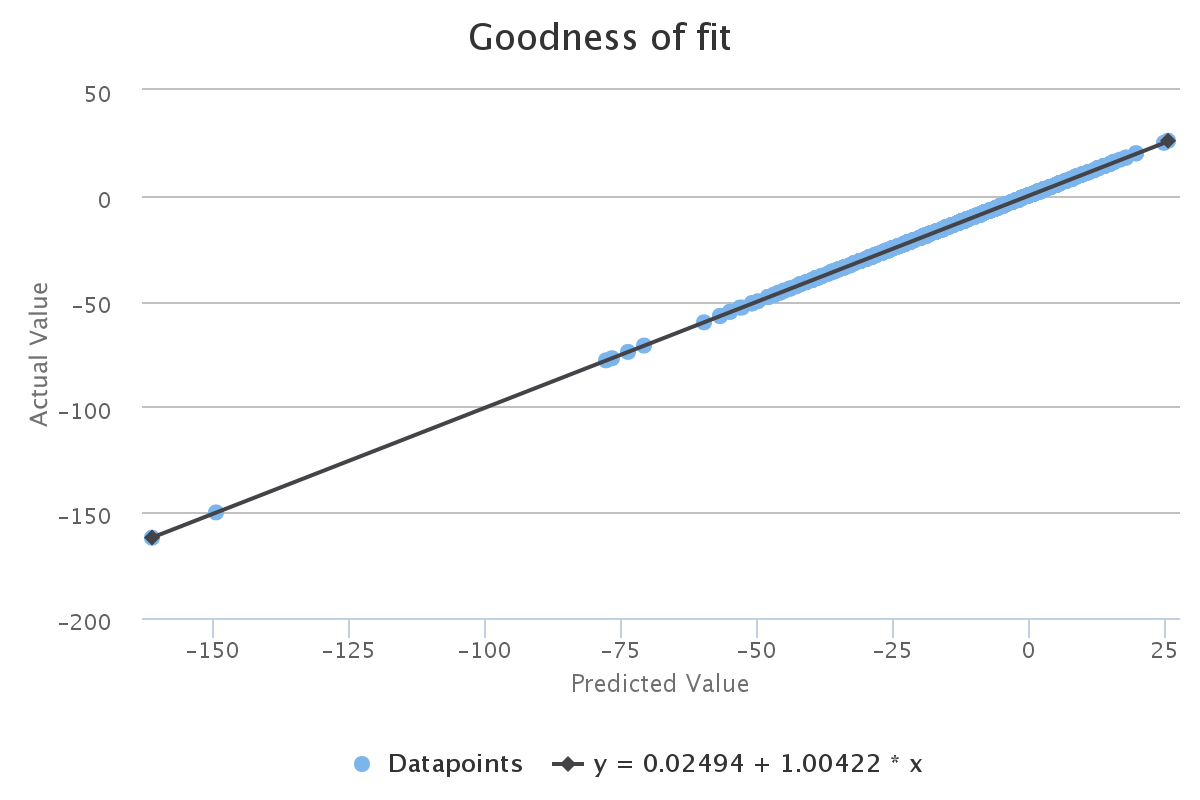
\includegraphics[width=0.45\hsize]{fbm-fit}
\label{fig:plots}
\end{tabular}
\mycaption{Performance of GPs model on Omni data \ Top: RBF kernel \ Bottom: FBM kernel}

\setlength{\arrayrulewidth}{1mm}
\setlength{\tabcolsep}{18pt}
\renewcommand{\arraystretch}{2.5}
{\rowcolors{2}{cwired!45}{cwired!35!}
\begin{tabular}{ |p{5cm}|p{5cm}|p{5cm}|p{5cm}|p{5cm}|  }
\hline
Kernel & Model Size: Train, Test & MAE & RMSE & $R^2$\\
\hline
RBF  & $300$,$1000$ & $1.5044$ & $6.9752$ & $0.7925$ \\
FBM  & $300$,$1000$ & $0.0312$ & $0.0461$ & $0.9999$ \\
\hline
\end{tabular} 
}
\vspace{\baselineskip}

The two models are then trained and tested on sub-sampled versions of the Omni data for the years 2007 and 2006 respectively. Figure \ref{fig:plots} compares the residual histograms and goodness of fit for both models. The results in figure 3 and the table above show that:
\begin{itemize}
    \item Although the RBF based model gives a satisfactory fit, it performs poorly in predicting outlying events like geomagnetic storms ($Dst \leq -100 nT$)
    \item From the residual histograms it can be observed that the FBM based GP model provides more robust Dst predictions in greatly varying solar wind conditions. 
\end{itemize}

\end{multicols}

\end{poster}

\end{document}
